\documentclass{article}
\usepackage{hyperref}
\usepackage{geometry}
\usepackage{amsmath}
\usepackage{graphicx}
\geometry{a4paper, margin=1in}

\title{Software Requirements Specification (SRS) \\ ArmSpace Project}
\author{Your Name}
\date{June 14, 2025}

\begin{document}

\maketitle

\tableofcontents

\section{Introduction}
\subsection{Purpose}
This document defines the software requirements specification (SRS) for the \textbf{ArmSpace} project. It outlines the functionality, interfaces, constraints, and testing strategies required for the initial version of the system.

\subsection{Scope}
ArmSpace is a software tool designed to process structured input data, perform calculations via a computation engine, and provide motor control commands in JSON format.

\subsection{Definitions and Abbreviations}
\begin{itemize}
    \item \textbf{SRS}: Software Requirements Specification
    \item \textbf{JSON}: JavaScript Object Notation
    \item \textbf{CMake}: Cross-platform build system
    \item \textbf{gtest}: Google Test framework
    \item \textbf{Quaternion}: A mathematical representation for rotation, avoiding gimbal lock.
\end{itemize}

\section{Overall Description}
\subsection{System Architecture Overview}
The system consists of multiple **modules** working together:

\begin{itemize}
    \item \textbf{Input Parser}: Validates and processes JSON input files.
    \item \textbf{Computation Engine}: Handles quaternion-based calculations and motor tick conversion.
    \item \textbf{Logging System}: Uses \textbf{spdlog} for structured error reporting.
    \item \textbf{Output Generator}: Produces JSON-formatted motor control values.
\end{itemize}

\subsection{Architecture Diagram}
\begin{figure}[h]
    \centering
    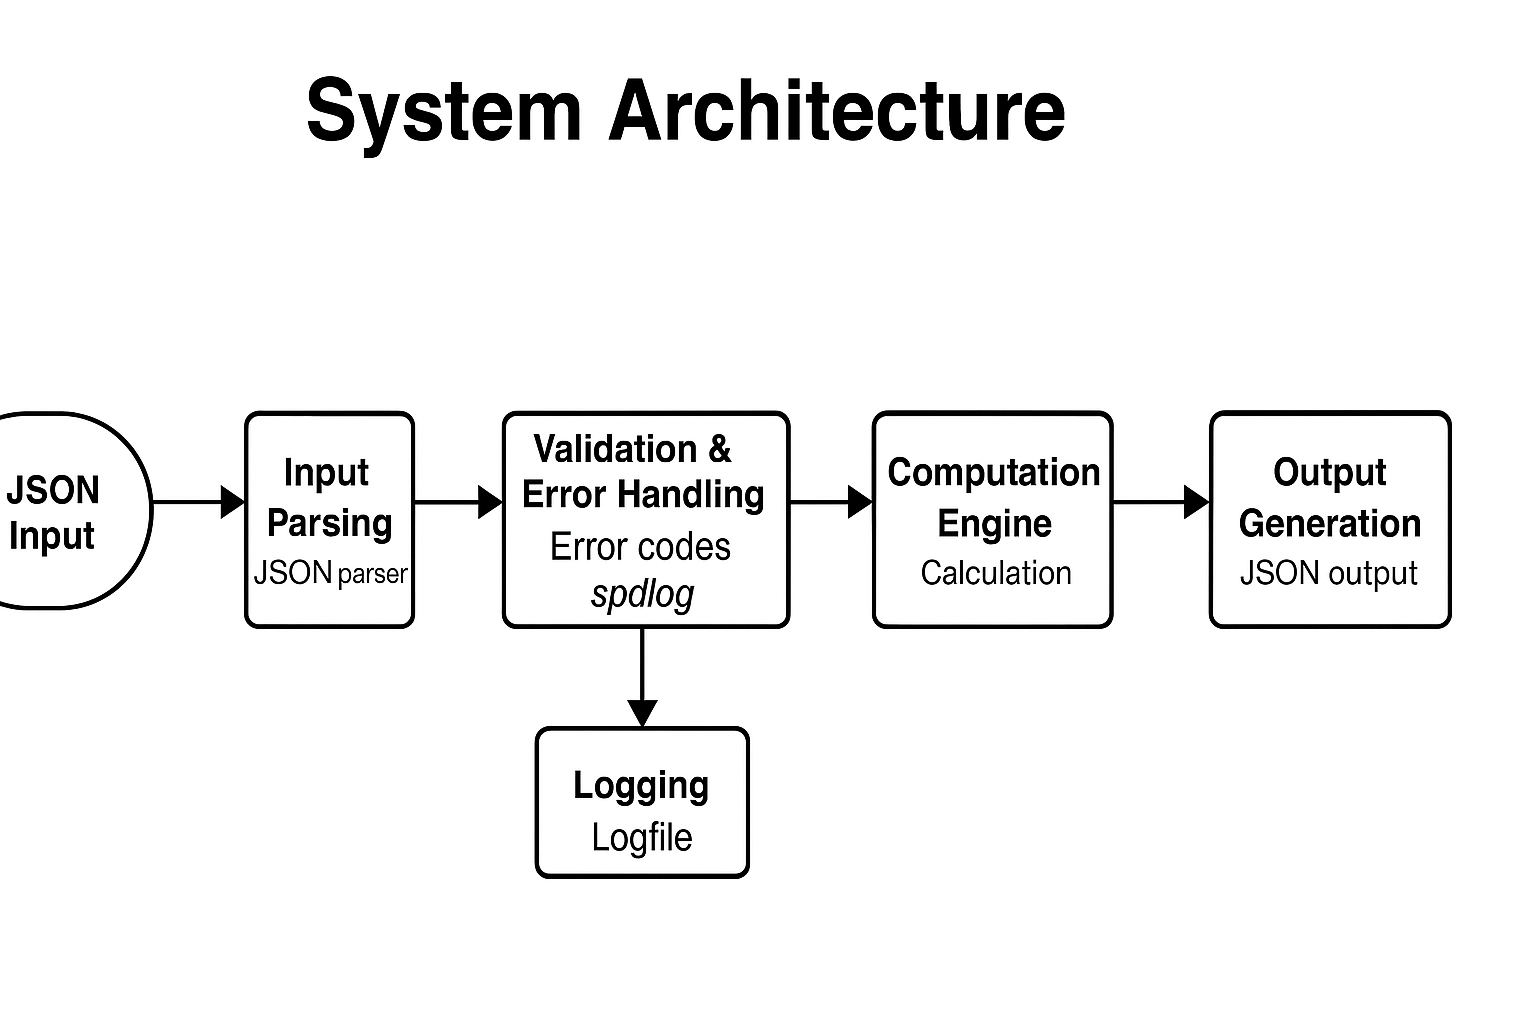
\includegraphics[width=0.8\textwidth]{architecture_diagram.png}
    \caption{ArmSpace System Architecture}
\end{figure}

\subsection{Supported Platforms}
ArmSpace is designed to run on:
\begin{itemize}
    \item **Linux**
    \item **macOS**
    \item **Windows**
\end{itemize}
Future versions may be ported to additional platforms.

\subsection{Constraints}
\begin{itemize}
    \item Implemented in C++
    \item Uses \textbf{nlohmann/json} for JSON parsing and writing
    \item Uses \textbf{spdlog} for logging
    \item Uses \textbf{CMake} as the build system for cross-compiling to Windows
    \item Input and output in JSON format
    \item Command-line interface (CLI) for the current version
\end{itemize}

\section{JSON Format Specification}
\subsection{JSON Input Format}
The system expects a structured JSON input, describing joints, motors, and arm segments.

\begin{verbatim}
{
    "robot_name": "ArmSpaceBot",
    "joints": [
        {
            "name": "shoulder",
            "position": [0, 0, 0],
            "motors": [
                {
                    "name": "shoulder_motor_x",
                    "rotation_axis": [1, 0, 0],
                    "ticks_per_revolution": 1000
                },
                {
                    "name": "shoulder_motor_z",
                    "rotation_axis": [0, 0, 1],
                    "ticks_per_revolution": 1200
                }
            ],
            "arm_segment": { "length": 10, "direction": [1, 0, 0] }
        },
        {
            "name": "elbow",
            "position": [10, 0, 0],
            "motors": [
                {
                    "name": "elbow_motor_y",
                    "rotation_axis": [0, 1, 0],
                    "ticks_per_revolution": 1100
                },
                {
                    "name": "elbow_motor_x",
                    "rotation_axis": [1, 0, 0],
                    "ticks_per_revolution": 900
                }
            ],
            "arm_segment": { "length": 10, "direction": [1, 0, 0] }
        }
    ],
    "desired_position": [10, 7, 5]
}
\end{verbatim}

\subsection{JSON Output Format}
The system calculates movements based on quaternion-based rotations and outputs motor tick values.

\begin{verbatim}
{
    "motor_ticks": [
        { "name": "shoulder_motor_x", "ticks": 97 },
        { "name": "shoulder_motor_z", "ticks": 82 },
        { "name": "elbow_motor_y", "ticks": 100 },
        { "name": "elbow_motor_x", "ticks": 105 }
    ],
    "status": "adjusted",
    "final_position": [10, 6.9, 4.9]
}
\end{verbatim}

\section{Error Handling}
\subsection{Error Reporting and Logging}
Standardized error codes ensure structured fault recovery.

\begin{table}[h]
\centering
\begin{tabular}{|c|l|p{8cm}|}
\hline
\textbf{Error Code} & \textbf{Message} & \textbf{Description} \\
\hline
ERR001 & Invalid Arm Length & A joint position does not match the expected length \& direction. \\
\hline
ERR002 & Disconnected Joint & A joint is not properly connected to the sequence. \\
\hline
ERR003 & Malformed JSON & The input structure is incorrect or missing required fields. JSON parsing failed. \\
\hline
ERR004 & Motor Data Missing & A motor definition is missing configurations, preventing tick calculation. \\
\hline
ERR005 & Unsupported Joint Count & The number of joints exceeds the maximum limit (future constraint: 6). \\
\hline
ERR006 & Invalid Rotation Axis & A motor has an incorrectly formatted rotation axis (should be a unit vector). \\
\hline
ERR007 & Quaternion Calculation Failure & Rotation computations failed due to incorrect vector inputs. \\
\hline
ERR008 & Tick Calculation Overflow & The computed tick value exceeds the allowed motor range. \\
\hline
\end{tabular}
\caption{Complete error code table for validation and computation}
\end{table}

\subsection{JSON Error Response Format}
If an error occurs, the system returns a structured JSON error message.

\begin{verbatim}
{
    "error": "Invalid arm length",
    "details": "Joint 'elbow' is not reachable from 'shoulder' based on defined segment length."
}
\end{verbatim}

\section{Mathematical Formulation}
\subsection{Quaternion-Based Rotation Computation}
A quaternion is defined as:


\[
q = \cos(\theta/2) + \sin(\theta/2) \cdot (x, y, z)
\]



\subsection{Applying Quaternion Rotation}
Given an initial vector \( P \), we apply the quaternion transformation:


\[
P' = q P q^{-1}
\]



\section{Performance Considerations}
Optimization monitoring will focus on:
\begin{itemize}
    \item **Execution Speed**
    \item **Memory Usage**
    \item **Algorithm Efficiency**
\end{itemize}

\end{document}
